\documentclass[../ro-fa-lab.tex]{subfiles}
\usepackage{hyperref}
\usepackage{graphicx}   % package for including images
\usepackage{xcolor}     % used by listings
\usepackage{listings}   % for nicely formatted code blocks
\lstset{
    language=C++,                   % language (adjust if needed)
    basicstyle=\ttfamily\small,     % monospace font, smaller size
    keywordstyle=\color{blue},      % keywords in blue
    commentstyle=\color{gray},      % comments in gray
    stringstyle=\color{red},        % string literals in red
    showstringspaces=false,         % don’t show special string spaces
    numbers=left,                   % line numbers on the left
    numberstyle=\tiny\color{gray},  % style for line numbers
    frame=single,                   % frame around the code block
    breaklines=true,                % automatically break long lines
    breakatwhitespace=true,         % break at whitespace if possible
    tabsize=2                       % tab size
}

\hypersetup{
    pdftitle={(EN) Errors},   % The title shown in the browser tab
    pdfauthor={},                    % Your name or organization
    pdfsubject={},                   % A brief description
    pdfkeywords={}
}

\begin{document}

\section{\textbf{Error Fix}}\label{errors}

\subsection{Profiler + VS Code Error}\label{profiler-vscode-error}

In the file \texttt{Profiler.h}, you have the following lines starting at line 11:

\begin{lstlisting}
// OS detection
#if defined(WIN32) || defined(_WIN32) || defined(__WIN32__) || defined(__NT__)
    #define PROFILER_WINDOWS
#elif __APPLE__
    #define PROFILER_OSX
#elif __linux__
    #define PROFILER_LINUX
#endif

#ifdef PROFILER_WINDOWS
    #include <Windows.h>
    #include <Shellapi.h>
#else
    #include <unistd.h>
#endif
\end{lstlisting}

You should modify them as follows:

\begin{lstlisting}
// OS detection
#if defined(__MINGW32__) || defined(__CYGWIN__)
    #define PROFILER_VSCODE
#elif defined(WIN32) || defined(_WIN32) || defined(__WIN32__) || defined(__NT__)
    #define PROFILER_WINDOWS
#elif defined(__APPLE__)
    #define PROFILER_OSX
#elif defined(__linux__)
    #define PROFILER_LINUX
#endif

#if defined(PROFILER_WINDOWS) || defined(PROFILER_VSCODE)
    #include <Windows.h>
    #include <Shellapi.h>
#else
    #include <unistd.h>
#endif
\end{lstlisting}

Below are the screenshots (approximately 80\% of text width), framed as figures:

\begin{figure}[htbp]
    \centering
    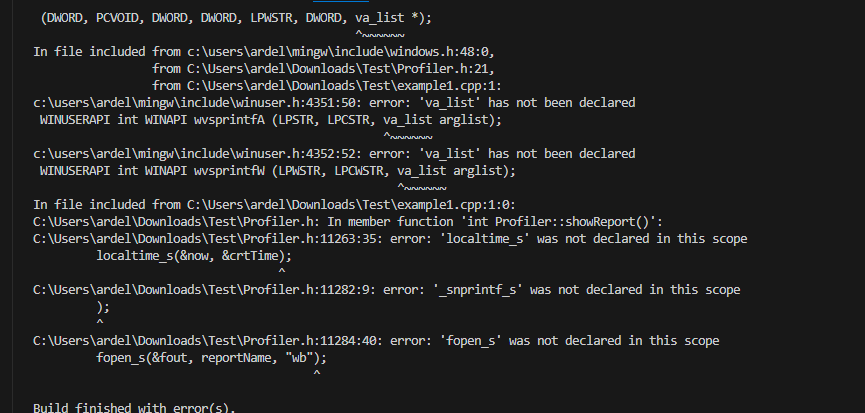
\includegraphics[width=0.8\textwidth]{./Resources/error_fix/image1.png}
    \caption{Initial error in VS Code Profiler}
    \label{fig:error1}
\end{figure}

\begin{figure}[htbp]
    \centering
    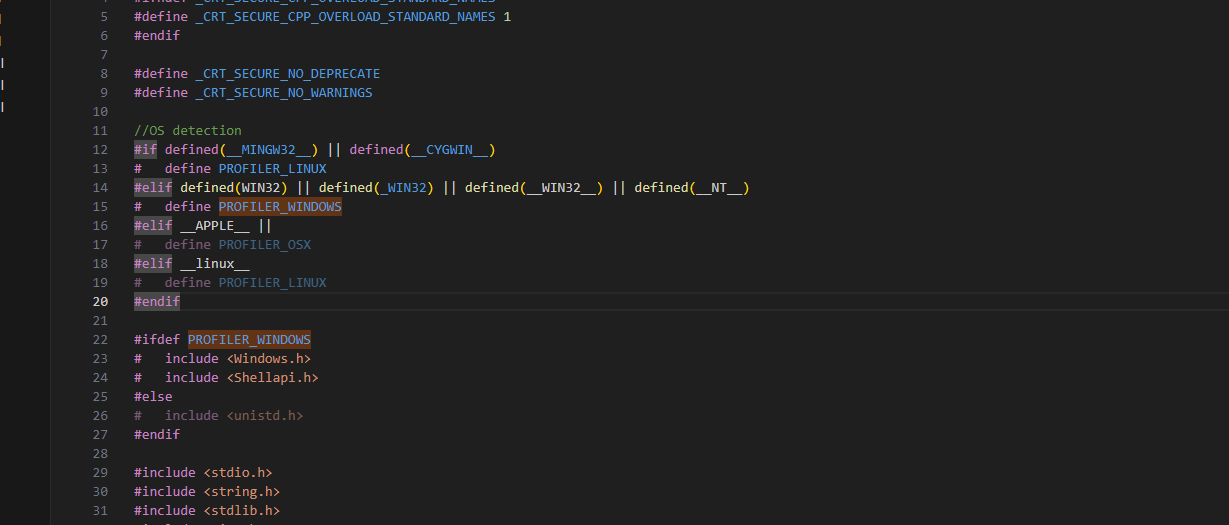
\includegraphics[width=0.8\textwidth]{./Resources/error_fix/image2.png}
    \caption{Original screenshot (before fix)}
    \label{fig:error2}
\end{figure}

\begin{figure}[htbp]
    \centering
    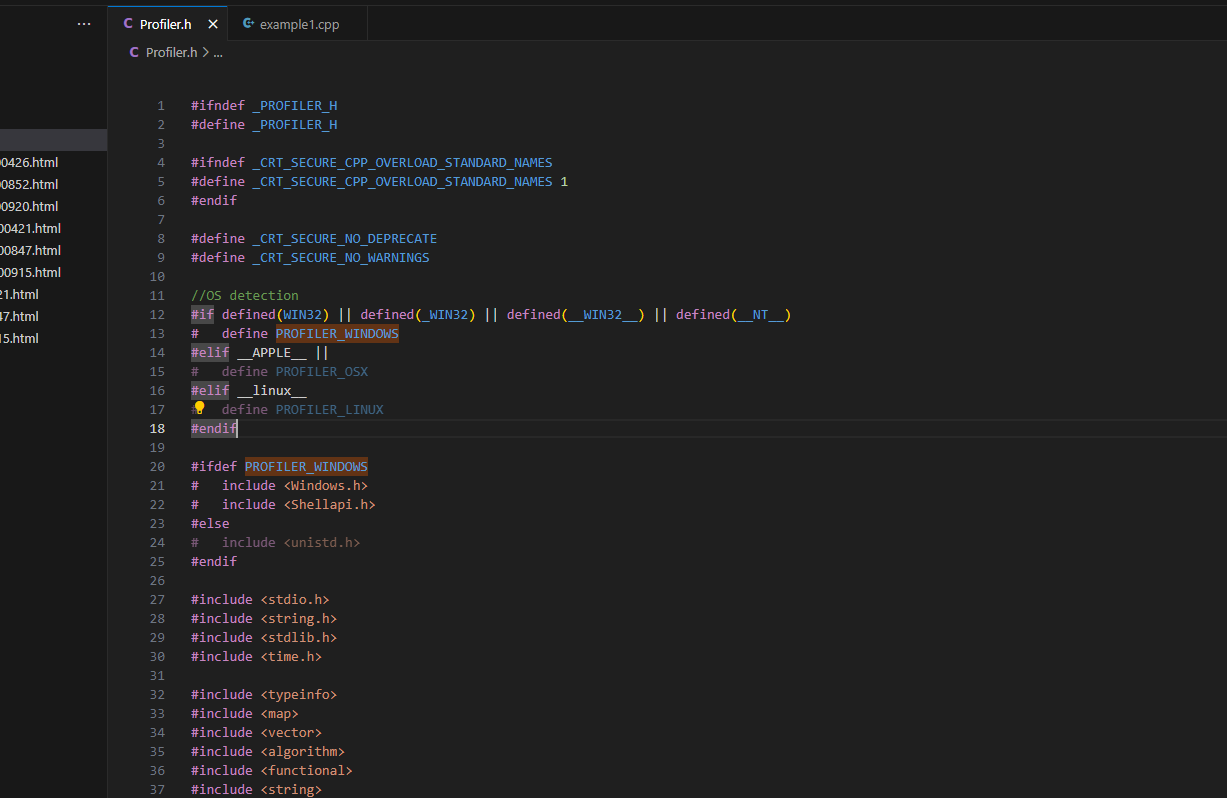
\includegraphics[width=0.8\textwidth]{./Resources/error_fix/image3.png}
    \caption{Screenshot after update (after fix)}
    \label{fig:error3}
\end{figure}

\end{document}
